\documentclass[a4paper]{article}
\usepackage[francais]{babel}
\usepackage[utf8]{inputenc}
\usepackage[toc,page]{appendix} 
\usepackage[T1]{fontenc}
\usepackage{graphicx}
\usepackage{fancyhdr}
\pagestyle{fancy}

% définir les entêtes et pieds de page
\lhead{Master Bioinformatique}
\rhead{Université Claude Bernard Lyon 1}
\renewcommand{\footrulewidth}{0.4pt}
\lfoot{UE Projet 2}
\rfoot{Février 2017}

% définir le titre et les auteurs sur la couverture
\title{{\sc \large Cahier des charges}\\
\bf Un site web interactif pour une meilleure compréhension de l’histoire évolutive des espèces}
\author{ShangNong {\sc Hu}\and Valentin {\sc Reymond}\and Grégoire {\sc Siekaniec}\and Krystian {\sc Valenducq}}
\date\today

% pour que la numérotation commence à partir de la deuxième page
\setcounter{page}{0}


\begin{document}

\begin{figure}[!t]
	\centering
	
\includegraphics[width=6cm]{ucbl.png}
	\hspace{\fill}
	
\includegraphics[width=2cm]{lbbe.png}
\end{figure}

\maketitle
% couverture sans numérotation
\thispagestyle{empty}

\begin{figure}[!b]
	\centering
	
\includegraphics[width=6cm]{logo.png}
\end{figure}

\newpage

\tableofcontents
\newpage


\section{Contexte biologique}
	\paragraph{}
	La vie sur Terre est apparu il y a quelques milliards d'années. Il a fallut de nombreuses étapes pour que cette grande histoire parvienne jusqu'à l'Homme et ses espèces contemporaines. Cette histoire est parsemée de nombreuses péripéties qui ont résulté par l'apparition et la disparition de très nombreuses espèces. Ces variations sont dues à de nombreuses extinctions qui ont eu lieu au cours des temps géologiques. En revanche ces bouleversements dans l'histoire de la Vie restent à l'heure actuelle très floues quant à leur intensité et leur origine.

	\paragraph{}
	De nos jours, le grand public adopte une vision biaisée de l'évolution, tel qu'il existe qu'une seule extinction qui a été celle des dinosaures. Alors que d'après les connaissances actuelles, on peut recenser jusqu'à sept extinctions massives dont celle des dinosaures est la plus récente.
	% à verifier le nombre

	\begin{figure}[!h]
		\centering
		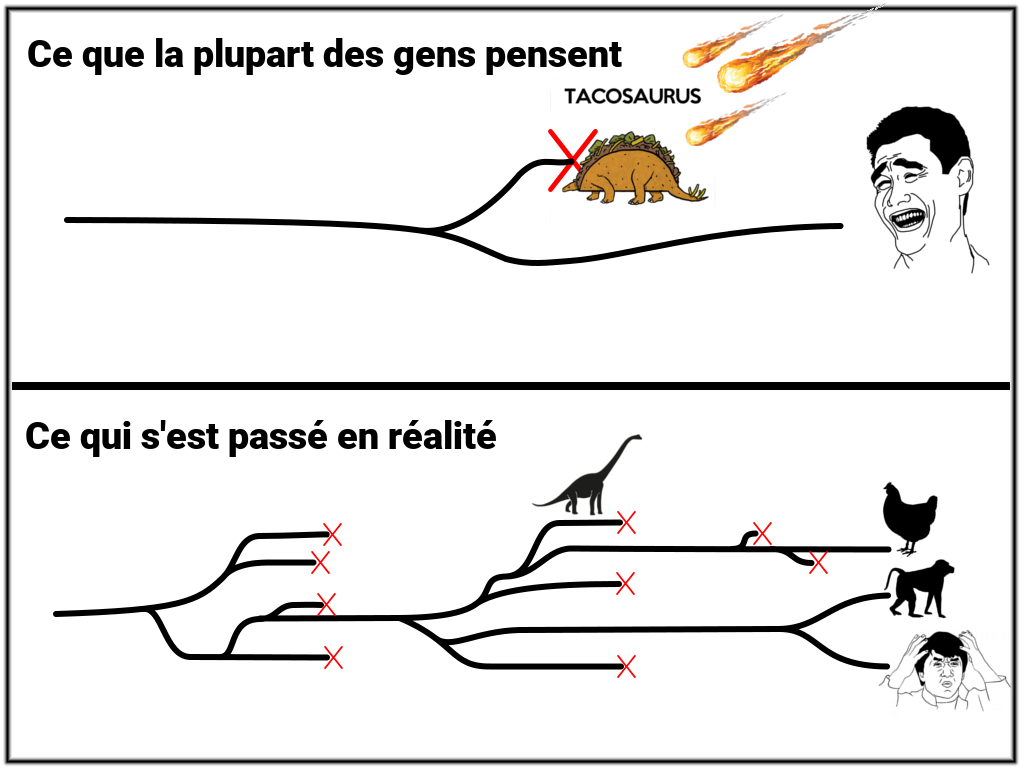
\includegraphics[width=12cm]{illustr1.png}
		\caption{La vision biaisé face à la connaissance actuelle.}
		\label{comic1}
	\end{figure}

	\paragraph{}
	Les trois chercheurs de l'Équipe Bioinformatique, Phylogénie et Génomique Évolutive à LBBE (UCBL Lyon 1), D. M. de Vienne, J.-P. Flandrois et L. Guéguen se sont interessés à la sensibilisation de ce grandes extinctions sur la biodiversité pour le grand public.

\section{Analyse des besoins}

	L'idée serait de retracer ces événements à l'aide d'un site web interactif, qui pourra par la suite être utilisé dans un but pédagogique (Université, Musée,\ldots).

	\subsection{Caractéristiques de la plateforme à mettre en place}
		\paragraph{}
		Le produit attendu sera un site web intéractif et responsive, c'est-à-dire accessible depuis différents appareils (Ordinateur, Tablette, Smartphone, \ldots).
		
		\paragraph{}
		Il sera chargé de présenter la \emph{timeline} de la vie, depuis l'apparition de la vie jusqu'à ce jour. Les événements de la vie seront présentés sous forme d'un arbre orienté horizontalement, et explorable depuis une barre de navigation.	De plus, cet outil permettra de mettre en lumière les différentes grandes crises qui ont eu un impact sur la densité des espèces au cours du temps. L'afficha mettra également l'accent sur les événements remarquables (tels que l'extinction des dinosaures). 
		
		\paragraph{}
		Nous souhaitons implémenter des informations supplémentaires concernant les taxons les plus représentatifs pour conserver un design intuitif et compréhensible.
		La navigation sera accompagnée d'une échelle de temps, afin que l'utilsiateur puisse se situer dans l'immensité des temps géologiques.
				

	\subsection{Outils utilisés pour répondre aux besoins}
		\paragraph{}
		Ce site sera réalisé à l'aide d'outils de développement web, à savoir les langages HTML5 / CSS3, ainsi que Javascript. Ces trois langages permettront de mettre en place la structure visuelle du site.
		En parrallèle nous utiliserons le framework graphique D3.js qui nous permettra d'afficher l'arbre, la chronologie, ainsi que les diverses informations. Ce framework est constitué de multiples packages différents qui donnent lieu à des représentation graphiques très riches. Nous allons également utiliser un framework, dénommé W3.CSS, qui nous permettra de rendre notre site internet responsive. Il sera donc consultable sur la pluspart des appareils disponible.

		\paragraph{}
		Pour générer notre arbre nous avons recours à un script Python en version 2.7. Nous utilisons cette version pour pouvoir obtenir des représentation graphique dans une fenêtre à l'aide de la bibliothèques Matplotlib. Cette bibliothèque n'étant pas encore bien fonctionnelle sur la version 3 de Python, nous sommes donc rester sur la version 2.7.
	
	\subsection{Ordre de priorité}
		\paragraph{}
		Il est important de définir un ordre de priorité dans la gestion des tâches pour la réalisation de ce projet. Nous disposons en effet d'un temps imparti relativement court.

		\paragraph{}
		En première approche nous devrons élaborer un script pour générer un arbre qui soit le plus représentatif de l'histoire évolutive de la vie sur Terre. Cet arbre devra bien montrer l'existence des grandes extinctions. 
		En second lieu il faudra créer la monture de notre site, avec les différentes parties, notamment celle qui devra accueillir l'arbre. 
		Une fois la structure du site terminé, nous devrons intégrer notre arbre avec des scripts javascript, notamment avec D3.js, pour obtenir les ramifications qui représenteront la biodiversité à un temps T. Cet arbre sera accompagné d'une échelle des temps géologiques, qui nous servira à nous situer dans l'histoire évolutive.

		\paragraph{}
		Enfin, s'il nous reste du temps, nous pourrons peaufiner notre site en y ajoutant des options complémentaires, comme par exemple le taux d'oxygène présent lors d'une période particulière, ou encore les épisodes d'ères glaciaires. Ces informations complémentaires peuvent apporter une meilleure compréhension des évenements qui ont fait varier la densité de la biodiversité au cours du temps.

\section{Analyse de l'existant}

	\subsection{Pixelspace}

	\subsection{TimeTree}

	\subsection{Onezoom}

	\subsection{Lifemap}

	\subsection{Algorithme de colonisation de l'espace}


\section{Déroulement du projet}
	
	\subsection{Planification}

		
		\subsubsection{Construction du coeur du programme}

			

		\subsubsection{Construction d’une interface graphique}

			

		\subsubsection{Construction des fonctionnalités facultatives}

			

	\subsection{Assurance qualité et tests du programme}

		

\section{Contraintes}

	\subsection{Contrainte temporelle}
		La date de rendu du cahier de charge est prévue le vendredi 17 février.
		La soutenance est prévue provisoirement le vendredi 24 mars, dont le délivrable devrait être rendu 2 jours avant.
		Le projet doit être développé dans une période de 1 mois.

	\subsection{Contraintes techniques}

		

	\subsection{Autres contraintes}

\section{Ouverture}
		
\newpage

\begin{appendices} 
	
\end{appendices} 

\end{document}
